\chapter{Numerical Experiments} 
\label{ch:experiments}

In this section we analyze the empirical performance of OGD, comparing it with the algorithm from the Online Portfolio Optimization literature that provides guarantees on total regret: OLU~\cite{das2013online}.
We also consider UP~\cite{cover1996universal} and ONS~\cite{agarwal2006algorithms}, because UP\footnote{
We used a na\"ive version of UP since the classic implementation required an unfeasible amount of time for the experiments.
Instead, we discretized the simplex with $10^4$ points and used the corresponding CRPs to approximate the integrals used by UP.} has the best theoretical guarantees on the regret $R_T$ and ONS because has both good theoretical guarantees on the regret on the wealth $R_T$ and is known to provide the best results regarding the regret on the wealth when analyzed empirically.

\begin{table}[ht!]\centering
\begin{tabular}{ |c||c|c|c|c| }
 \hline
 \multicolumn{5}{|c|}{Datasets} \\
 \hline
 Name & Market &Year Span & Rebalances & Assets\\
 \hline
 NYSE(O) & New York Stock Exchange  & 1962 - 1984  &5651&   36\\
 TSE & Toronto Stock Exchange & 1994 - 1998  & 1258   &88\\
 SP500 & Standard Poor's 500 & 1998 - 2003 & 1276&  25\\
 \hline
\end{tabular}
\caption{Description of the main datasets used that common in the Online Portfolio Optimization literature.}\label{tab:dataset}
\end{table}

Table \ref{tab:dataset} summarizes the datasets used for the experiments. All assets in the datasets are being anonymize to ensure to avoid common bias toward specific assets.
To compare the algorithms, we used mainly the NYSE(O) dataset, a well-known benchmark that has been previously used in several portfolio optimization research papers, and notably, in all the works which propose the algorithms here considered as baselines.
The NYSE(O) dataset spans $22$ years (between $1962$ and $1984$), for a total investment horizon of $T = 5651$ days ($\approx250$ working days per year).
In each experiment, we sampled a set of $N=5$ assets randomly chosen among the $36$ and ran the algorithms for the entire investment horizon $T$.
We ran $100$ independent experiments for the NYSE(O) datasets, $20$ and $50$ for the TSE and SP500 dataset respectively, and then we averaged the results. The choice of doing a great number of experiments is to stress the point that we are not concerned with the selection of assets to invest in, but only with the behavior of the algorithms with respect to transaction costs.
We considered different values for the transaction rate $\gamma \in \{ 0, 0.0005, 0.001, 0.003, 0.006, 0.01, 0.02, 0.04 \}$, including hight values of $\gamma$ to simulate highly illiquid markets.

To set the parameter $K$ of OGD, we used the learning rate $\eta_t$ prescribed by Theorem~\ref{thm:total_regret}, with $\epsilon_l = 0.8$ and $\epsilon_u = 1.2$, for which Assumption~\ref{ass:nojunk} holds in the dataset NYSE(O).
For ONS, we used $\eta = 0$, $\beta = 1$, $\delta = 1/8$, as suggested by the authors in~\cite{agarwal2006algorithms}.
We used $\alpha = 0.12$ and $\eta = 1.3$ for OLU, which is the best combination of parameters according to~\cite{das2013online}.
All algorithms have been initialized with $\mathbf{x}_1 = \frac{1}{N} \mathbf{1}$.

We used the Annual Percentage Yield (APY) as a metric, assuming $250$ working days per year and one update per day.
Formally, the APY for the wealth $W$ is defined as:
\begin{equation*}
    A(W) = W^{250/T} - 1,
\end{equation*}
where $W \in \{ W_T^C, \tilde W_T \}$ and are defined in equation \eqref{eq:l1_wealth} and \eqref{eq:realwealth} respectively.
$95\%$ confidence intervals for the mean have been computed with statistical bootstrapping and are depicted as semi-transparent areas.

\subsection{Results on the NYSE(O) dataset}

\begin{figure}[t!]
    \centering
    \subfloat[\label{fig:ex1}]{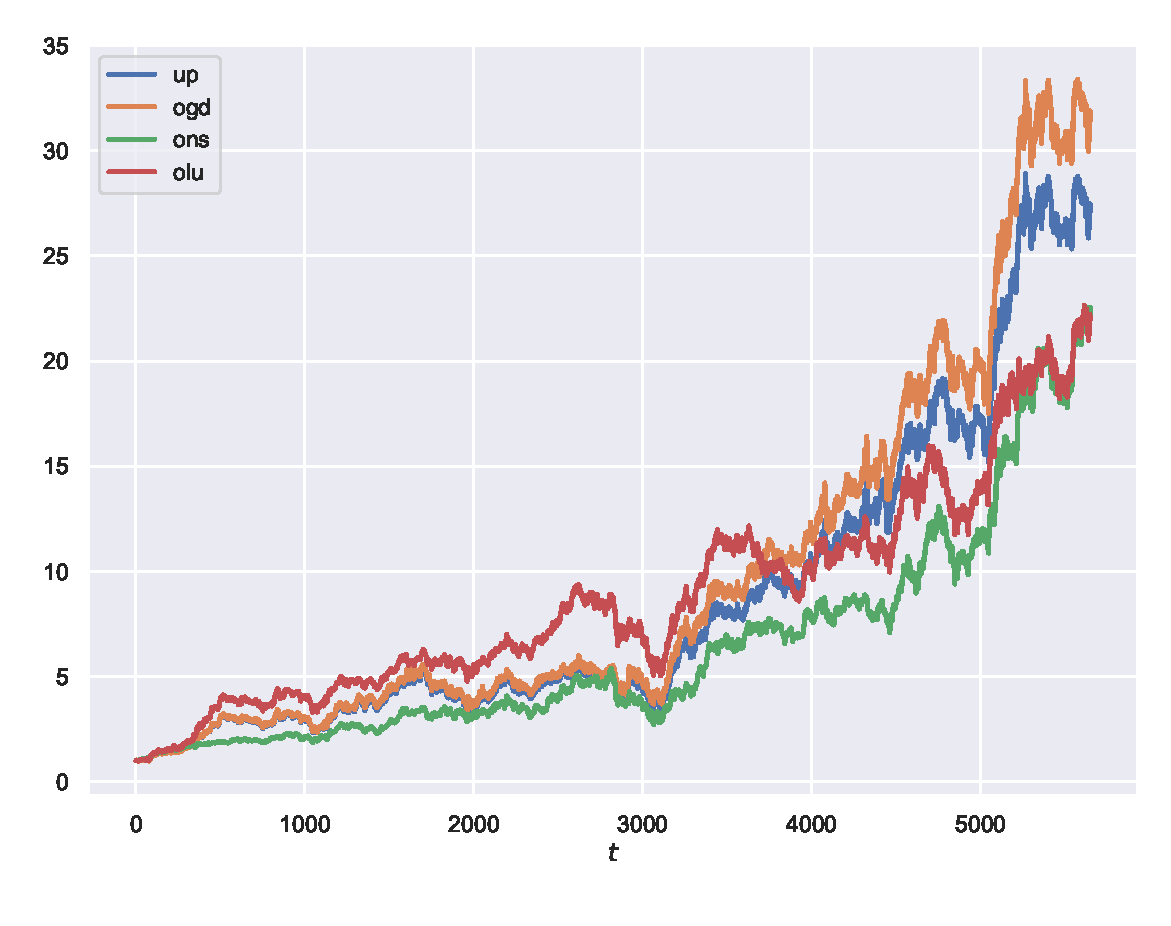
\includegraphics[width=0.48\textwidth,keepaspectratio]{img/fig_11.pdf}}
    \subfloat[\label{fig:ex2}]{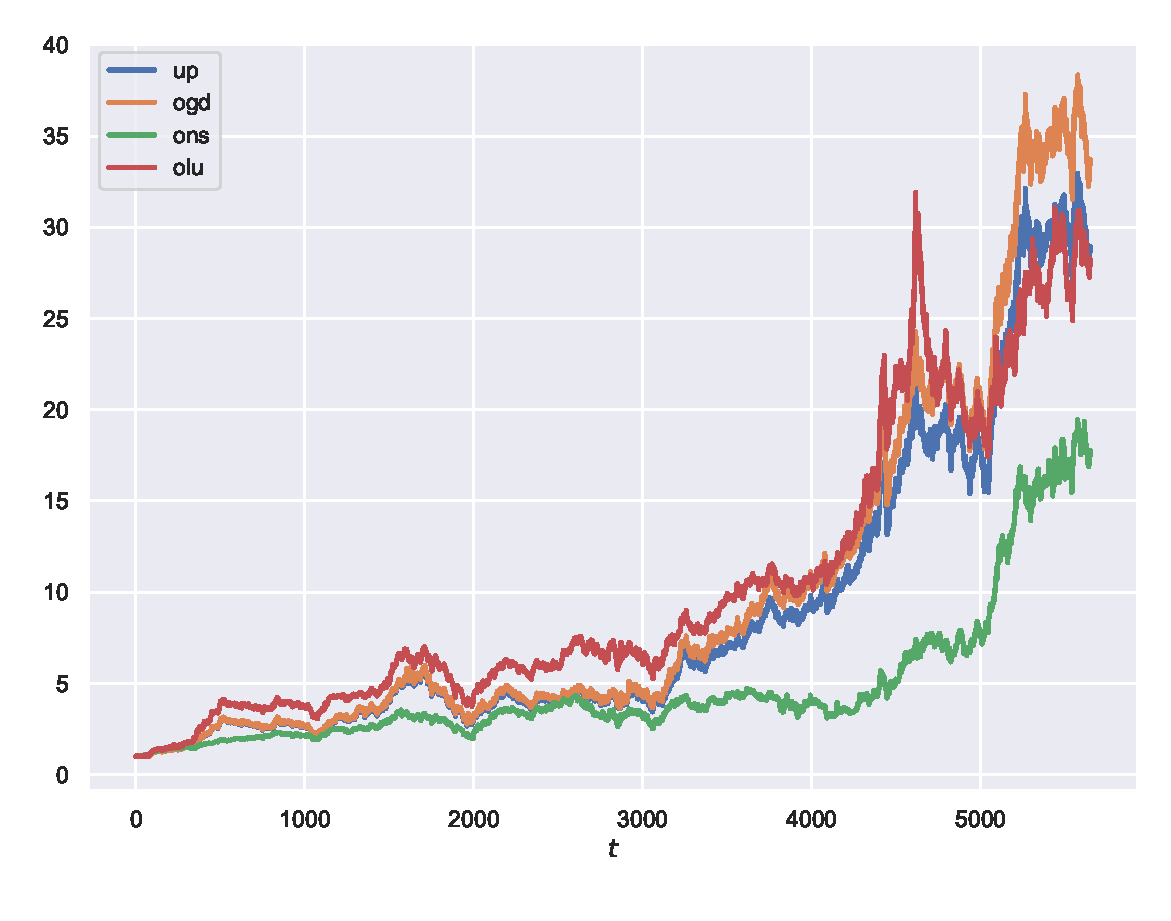
\includegraphics[width=0.48\textwidth,keepaspectratio]{img/fig_12.pdf}}
\caption{Wealth $W_T^C(\mathcal{A})$ on two runs of the NYSE(O) for $\gamma = 0$ (a), and $\gamma = 0.001$ (b).} \label{fig:algo_copmarison}
\end{figure}

Figure~\ref{fig:algo_copmarison} shows the evolution of the total wealth ${W}^C_t(\mathcal{A})$ of the different algorithms over the investment horizon in two specific runs, one without any cost ($\gamma = 0$) (Figure~\ref{fig:ex1}), and one with a transaction rate of $\gamma = 0.001$ (Figure~\ref{fig:ex2}).
In these two specific runs, OGD obtains a cumulative wealth larger than any other algorithm analyzed, suggesting that, in some settings, it might provide the best performance.
The results with $\gamma = 0$ suggest that OGD might be a viable solution even in the absence of costs.


\begin{figure}[ht!]
\centering
{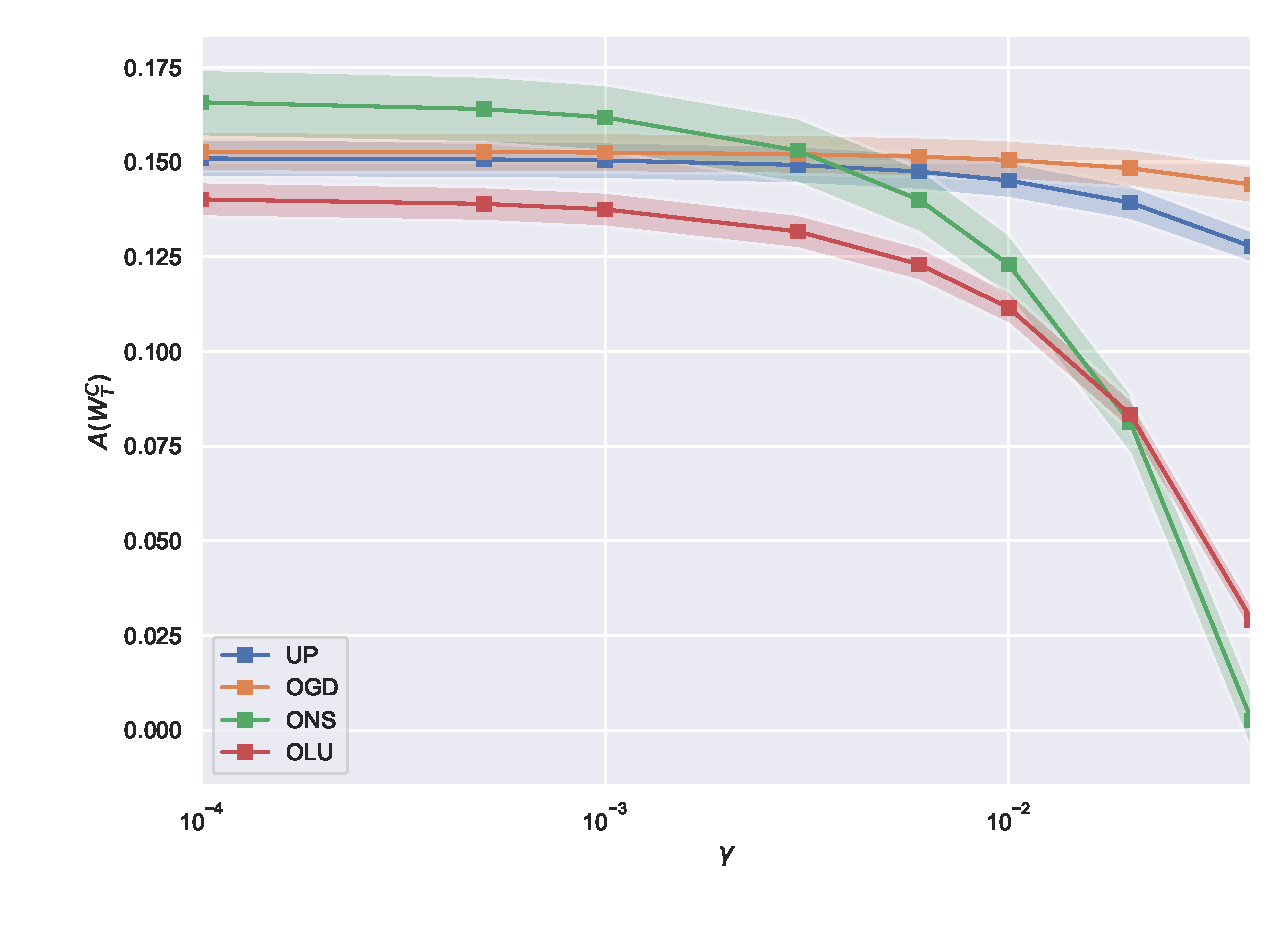
\includegraphics[width=0.80\textwidth,keepaspectratio]{img/fig_w_decay_l1.pdf}} 
\caption{Average APY computed on the wealth $W_T^C$ assuming the costs given by $C_T(\mathcal{A})$ for the NYSE(O) dataset.}
\label{fig:wealth_decay_l1}
\end{figure}

\begin{figure}[ht!]
\centering
{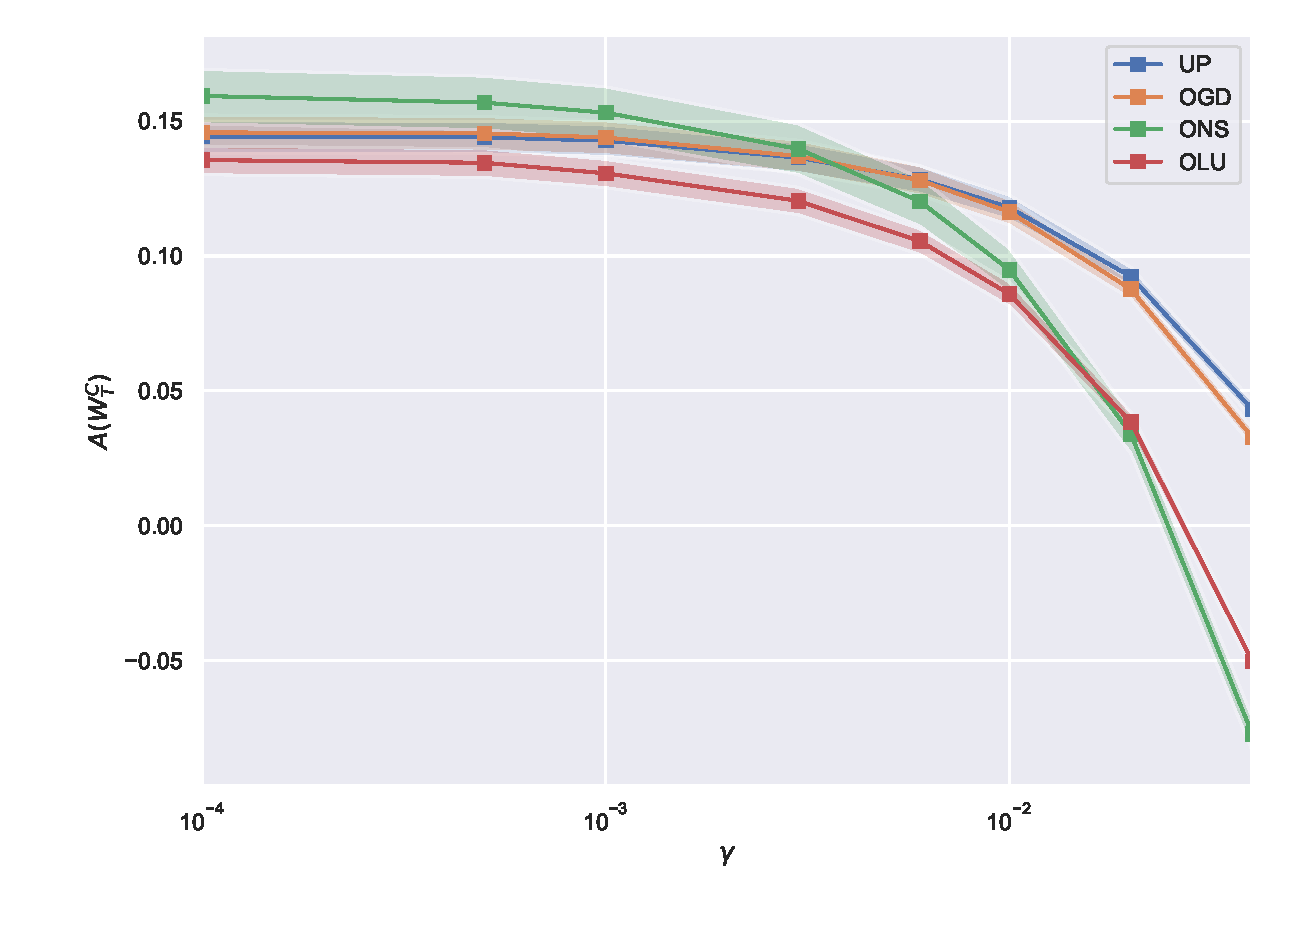
\includegraphics[width=0.80\textwidth,keepaspectratio]{img/fig_w_decay_true.pdf}} 
\caption{ Average APY computed on the wealth $\tilde{W}_T(\mathcal A)$ assuming the costs given by Equation~\eqref{eq:real_tc}, for the NYSE(O) dataset.}
\label{fig:wealth_decay_true}
\end{figure}

\begin{figure}[ht!]
\centering
{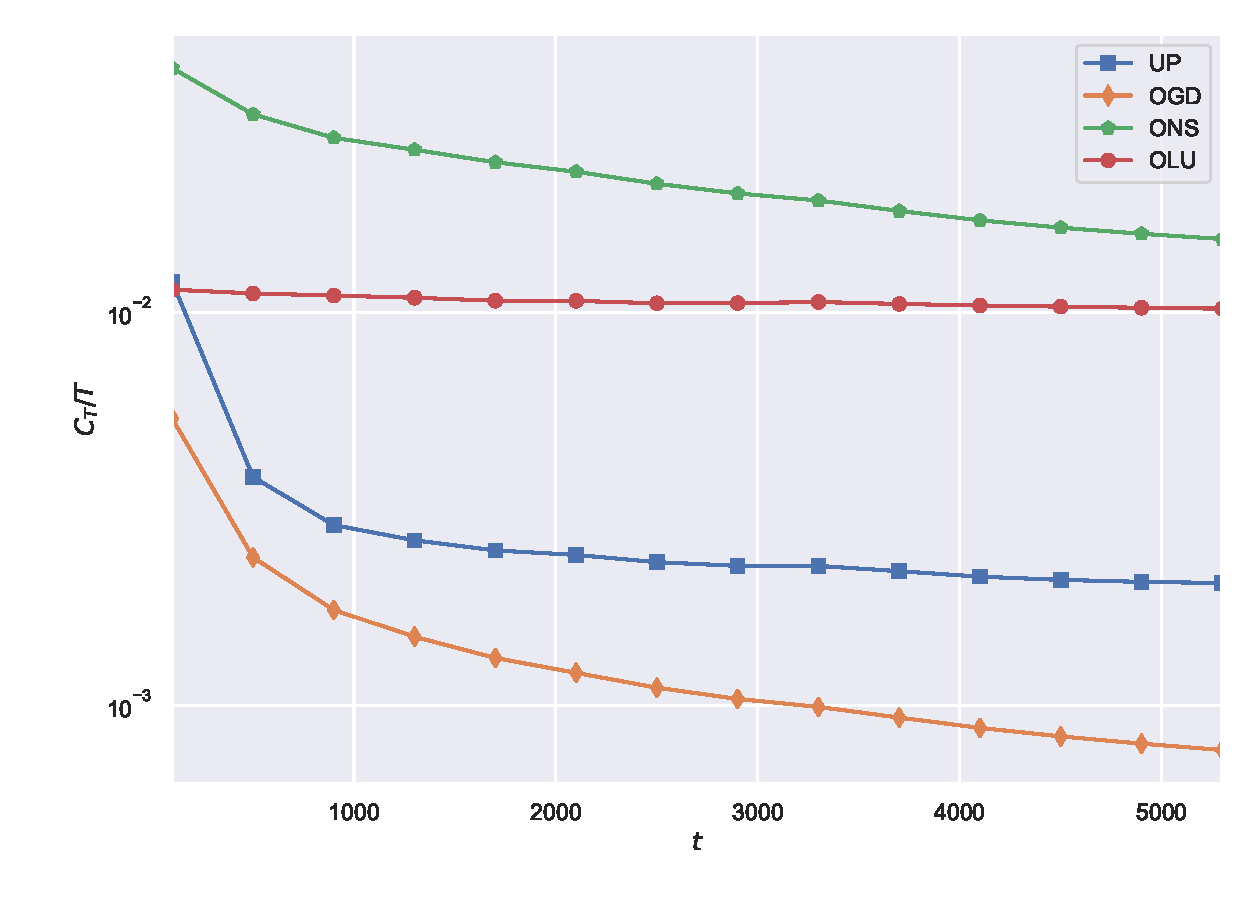
\includegraphics[width=0.80\textwidth,keepaspectratio]{img/fig_costs.pdf}}
\caption{Average costs $C_T(\mathcal{A})$ with $\gamma = 1$, for the NYSE(O) dataset.}
\label{fig:costs}
\end{figure}

In Figure~\ref{fig:wealth_decay_l1}, we present the results for the average APY, with the corresponding confidence intervals.
In particular, with no transaction costs ($\gamma = 0$), all the analyzed algorithms give similar results.
In this setting, ONS is the algorithm with the largest APY.
As we increase the transaction rate $\gamma$, OGD gets the largest APY, while OLU and ONS seem to be penalized by large transaction costs.
Conversely, the fact that the APY decreases from $\approx 0.15$ to $\approx 0.14$ suggests that OGD is effective at minimizing the costs $C_T(\mathcal{A})$.

Figure~\ref{fig:wealth_decay_true} considers the wealth $\tilde{W}_T(\mathcal{A})$, \emph{i.e.}, the one defined in Equation~\eqref{eq:realwealth}.
We notice that comparing these results with the ones obtained using $W_T^C$ (Figure~\ref{fig:wealth_decay_l1}), we have a smaller APY when $\gamma \gg 0$.
This suggests that, when applied to real-world cases, they might under-perform w.r.t.~what is expected from the theoretical results. 
In terms of $\tilde{W}_T(\mathcal{A})$, UP seems to perform slightly better than OGD, but the difference is not statistically significant for $\gamma < 0.04$.
ONS and OLU provide negative profits ($A(\tilde{W}_T) < 0$) for large values of transaction costs, \emph{e.g.}, for $\gamma = 0.04$ the APY becomes negative and, thus, the accumulated wealth is completely canceled out by the transaction costs.
From Figure~\ref{fig:wealth_decay_true}, we would be inclined to choose ONS for $\gamma \leq 0.003$, and OGD for $\gamma \geq 0.003$.

Figure~\ref{fig:costs} shows the averaged cost per round $C_t(\mathcal{A})/t$ and the corresponding confidence intervals, with $\gamma = 1$ (the value of $\gamma$ has been chosen to easily interpret how the regret on the costs behaves over time).
OGD is the algorithm that provides the lowest cost per round, which strengthens the claim of this work that OGD keeps transaction costs low.
The costs per round for OLU are approximately linear, as expected from the theory (see Section~\ref{sec:OLU}).
Conversely, the results for ONS, while not having any theoretical guarantee on $C_T(\mathcal{A})/T$, suggest that it has a cost per round of order $\mathcal{O}(\sqrt{T})$, but with a larger constant than OGD.
Finally, the costs of UP decrease slower than those of ONS and OGD.

\subsection{Results on the TSE and SP500 dataset}

\begin{figure}[ht!]
\centering
{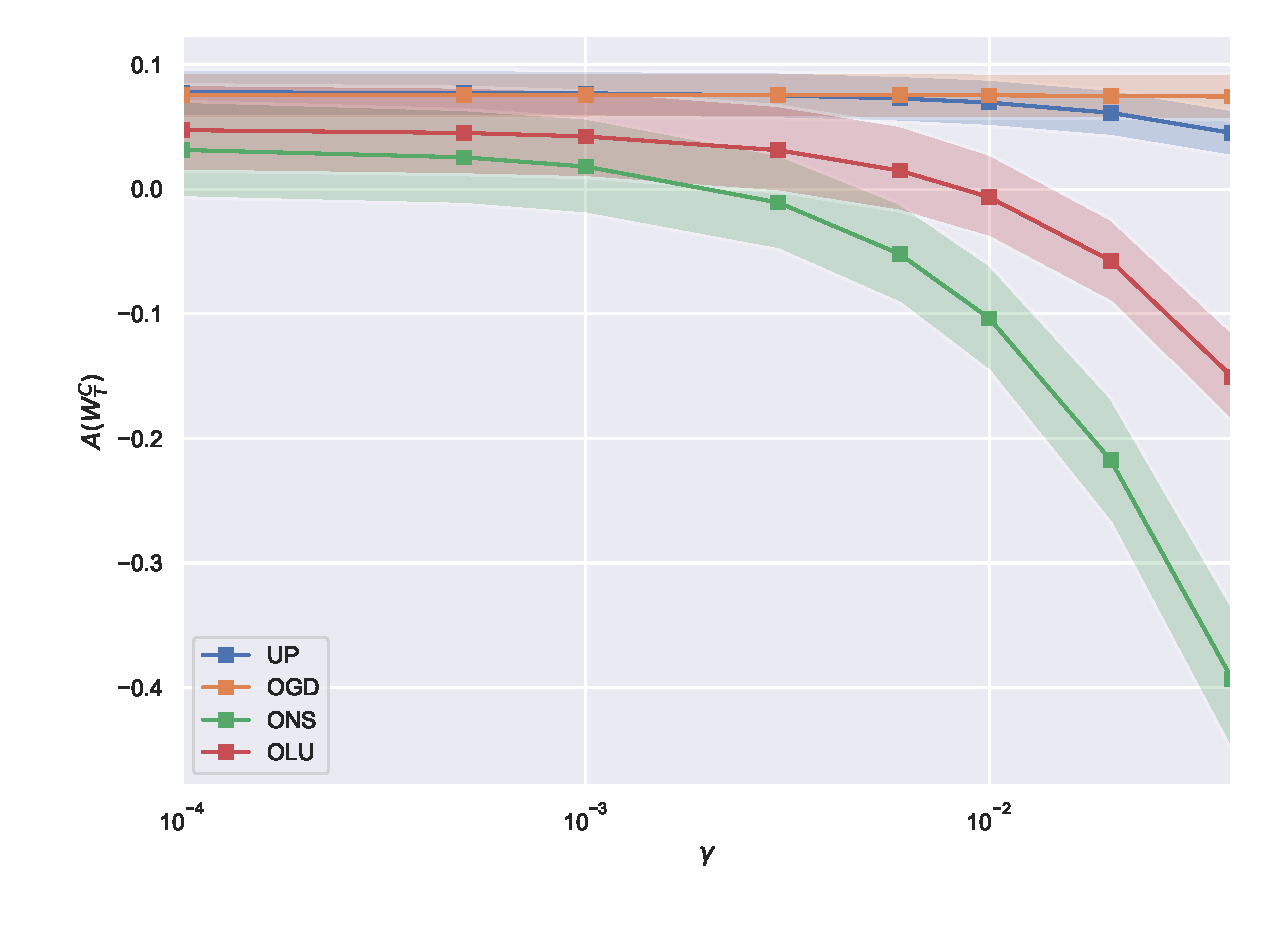
\includegraphics[width=0.80\textwidth,keepaspectratio]{img/fig_w_decay_l1_tse.pdf}} 
\caption{Average APY computed on the wealth $W_T^C$ assuming the costs given by $C_T(\mathcal{A})$ for the TSE dataset.}
\label{fig:wealth_decay_l1_tse}
\end{figure}

\begin{figure}[ht!]
\centering
{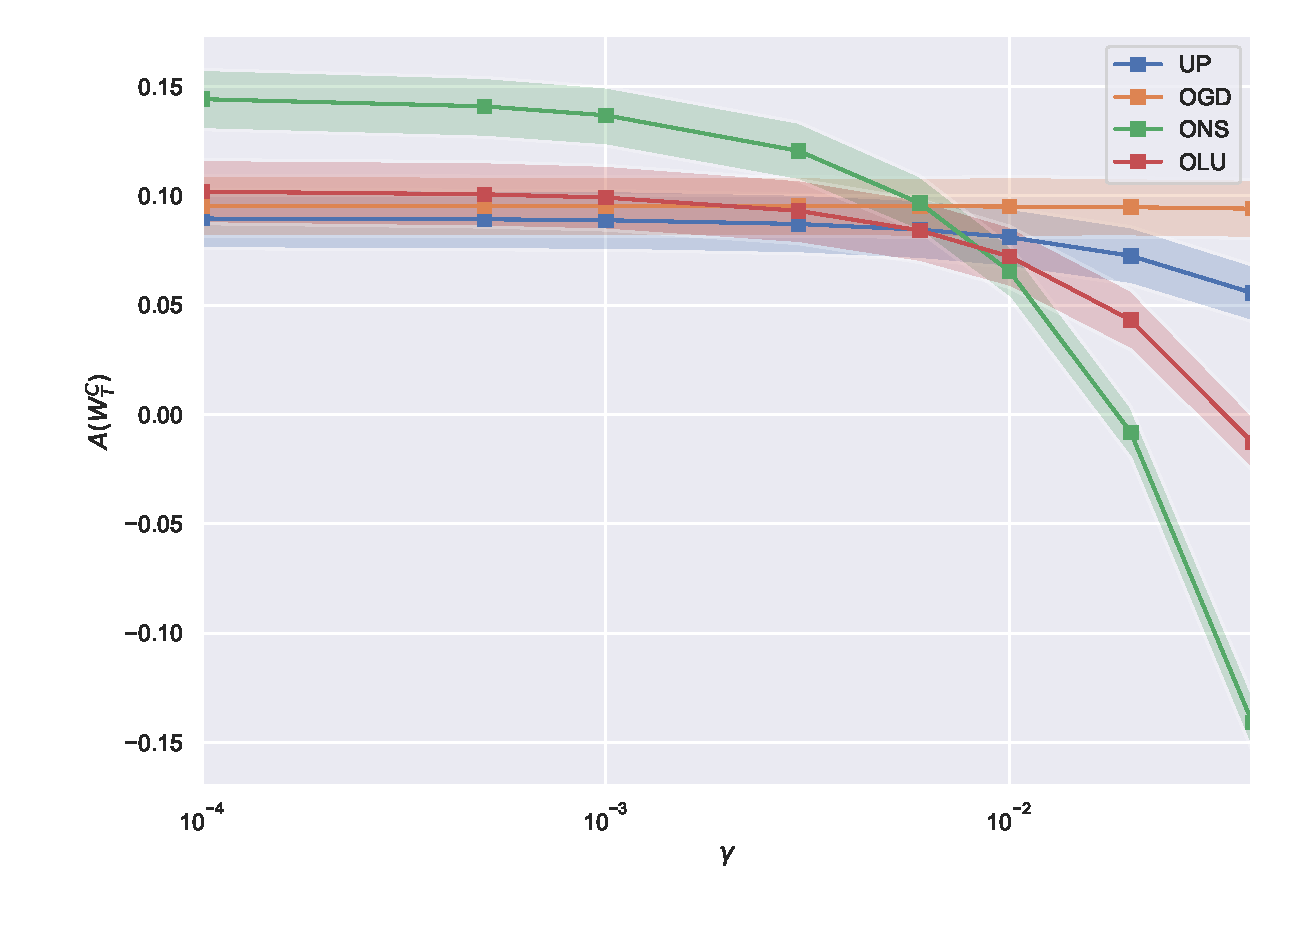
\includegraphics[width=0.80\textwidth,keepaspectratio]{img/fig_w_decay_l1_sp500.pdf}} 
\caption{Average APY computed on the wealth $W_T^C$ assuming the costs given by $C_T(\mathcal{A})$ for the SP500 dataset.}
\label{fig:wealth_decay_l1_sp500}
\end{figure}

In Figure \ref{fig:wealth_decay_l1_tse} and \ref{fig:wealth_decay_l1_sp500} present the results obtained on the TSE and SP500 datasets respectively, using the same approach we used for the NYSE(O) dataset.  The results obtained are in line with the one presented with the NYSE(O) dataset, i.e, the OGD algorithm performs better than the others for transaction rate greater than $0.003$, while it presents similar performance, in terms of APY, for smaller values of the transaction rate. Notably, in the SP500 dataset, ONS outperforms the other algorithms form small transaction rate $\gamma$, while in the TSE dataset, even for small values of the transaction rate $\gamma$, it is out-performed by the other algorithms.
